% 1. Dataset analysis
% Kaynak: notlar.md (Kararlar, Veri seti gözlemleri). Sayılar results/ altındaki dosyalardan.
% Bütçe: ~1 sayfa (Hafta 5'te eklenecek görsellerle birlikte).

\section{Dataset Analysis}\label{sec:dataset}

\paragraph{Source and licence}
I use the RAVDESS dataset~\cite{ravdess}, downloaded from its official Zenodo record~\cite{ravdesszenodo}. It contains recordings of 24 professional actors (12 female, 12 male) who say two lexically matched sentences, ``Kids are talking by the door'' and ``Dogs are sitting by the door'', with different emotions. The recordings were made under controlled studio conditions, and their emotional content was validated by 247 raters in the original study~\cite{ravdess}. The dataset is released under the CC BY-NC-SA 4.0 licence. I use it only for this non-commercial course project and I do not redistribute it, so the video files are not part of the code repository. After downloading, I checked all 24 archives against the MD5 checksums published on Zenodo.

\paragraph{Selected subset}
Every RAVDESS recording exists in three versions: audio-visual (modality~01), video-only (02) and audio-only (03). In this project the only input of the system is the camera image; no microphone is used. The tone of voice in which a person says a sentence therefore has no value for the system, and the emotion has to be recognised from the face alone. For this reason I kept only the video-only files. The audio-visual files contain exactly the same frames, so using them as well would count every clip twice. I also left out the song part of the dataset, because it covers only six of the eight emotions (surprise and disgust are missing) and has no recordings for one of the actors. The resulting subset has 1,440 clips, 60 per actor (Table~\ref{tab:dataset}). Each file name encodes the modality, emotion, intensity, sentence, repetition and actor, so I built the index of the dataset directly from the file names and checked all expected counts automatically.

\begin{table}[t]
\centering
\caption{Summary of the dataset used in this project.}
\label{tab:dataset}
\small
\begin{tabular}{@{}ll@{}}
\toprule
Property & Value \\
\midrule
Source & RAVDESS, Zenodo record 1188976 \\
Licence & CC BY-NC-SA 4.0 \\
Subset & Video-only (modality 02), speech \\
Actors & 24 (12 male, 12 female) \\
Clips & 1,440 (60 per actor) \\
Resolution & 1280$\times$720, H.264 \\
Frame rate & 29.97 fps \\
Clip length & 2.94--5.27 s (median 3.67 s) \\
Frames per clip & 88--158 (median 110) \\
Classes & 7 (calm merged into neutral) \\
Clips per class & neutral 288, others 192 each \\
Training set & 16 actors (960 clips) \\
Validation set & actors 3, 12, 21, 24 (240 clips) \\
Test set & actors 4, 6, 7, 23 (240 clips) \\
\bottomrule
\end{tabular}
\end{table}


All clips are H.264 videos with a resolution of $1280\times720$. Their measured frame rate is 29.97~fps (in the proposal I gave the nominal value of 30~fps). The clips are short, between 2.94 and 5.27~s (88--158 frames, median 110), so even the shortest clip has enough frames for the frame counts $T \in \{8, 16, 32\}$ that I plan to test.

\paragraph{Classes}
RAVDESS uses eight emotion labels. In the original labels, neutral has 96 clips, while calm and each of the other six emotions have 192 clips, because neutral was recorded at only one intensity. As planned in the proposal, I merged calm into neutral, because both are low-arousal (calm) expressions that look very similar on the face and both correspond to a resting expression of the avatar. After merging, neutral has 288 clips (96 + 192) and each of the other six classes has 192 clips (Figure~\ref{fig:classes}). Neutral is therefore 1.5 times larger than the other classes and makes up 20\% of the data. Because of this imbalance, I use the macro F1-score, which gives every class the same weight, as the main metric. Within every class, half of the clips come from male and half from female actors.

\begin{figure}[t]
\centering
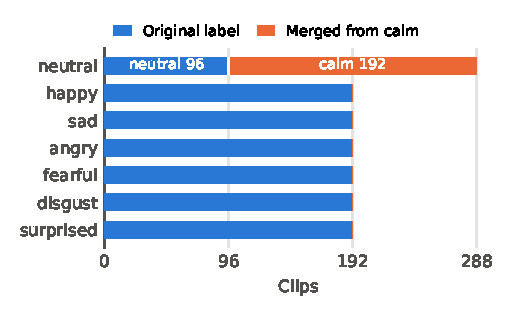
\includegraphics[width=\columnwidth]{class_distribution.pdf}
\caption{Number of clips per class. The neutral class is the union of the original neutral (96) and calm (192) clips.}
\label{fig:classes}
\end{figure}

% Hafta 5: her duygudan örnek yüz kırpması + bir klibin kare şeridi (tek şekil olarak birleştirilebilir)
% Hafta 5: klip süresi / kare sayısı histogramı
\todo{Week 5: sample face for each emotion, frame strip of one clip, clip length histogram.}

\paragraph{Actor-wise split}
If the clips were split at random, clips of the same actor would end up in both the training and the test data, and a model could score well by recognising the person instead of the emotion. In the live demo, however, the model will always see a person it has never seen before. For this reason I split the data by actor, so that all clips of an actor are used for only one purpose.

With only 24 actors, a test set of four actors would make the result depend strongly on which four people were chosen. I therefore divided the actors into six groups (folds) of four, each with two male and two female actors, using a fixed random seed (4206). For the final comparison, every model will be trained six times: each time a different fold is the test set, the next fold is the validation set and the remaining four folds (16 actors) are used for training. In this way every actor is tested exactly once, and I can report the mean and standard deviation of six results instead of a single number. Because every actor has the same number of clips per emotion, every fold is also class-balanced (48 neutral clips and 32 clips of each other class).

Training every experiment six times would take too long during development, so until the final comparison I use only the first of these six rounds as a fixed split: actors 4, 6, 7 and 23 for testing, actors 3, 12, 21 and 24 for validation and the remaining 16 actors for training (960 / 240 / 240 clips). The validation actors are used to follow the training; the test actors stay locked until model development is finished. The data loading code returns the test set only when this is requested explicitly, and all results in this report are on the validation actors.
